\documentclass[11pt]{article}
\usepackage[margin=0.9in]{geometry}
\usepackage[T1]{fontenc}
\usepackage{lmodern}
\usepackage{microtype}
\usepackage{amsmath,amssymb,bm}
\usepackage{booktabs,array}
\usepackage{graphicx}
\usepackage[round,authoryear]{natbib}
\usepackage{xcolor}
\usepackage[colorlinks=true,linkcolor=blue!45!black,citecolor=blue!45!black,urlcolor=blue!45!black]{hyperref}
\graphicspath{{../figures/}{figures/}}
\setlength{\parskip}{0.35em}
\setlength{\parindent}{0pt}
\setlength{\emergencystretch}{2em}
\allowdisplaybreaks[2]
\newcommand{\dd}{\mathrm d}
\newcommand{\ii}{\mathrm i}
\newcommand{\E}{\mathbb E}
\newcommand{\Ai}{\operatorname{Ai}}
\newcommand{\erfc}{\operatorname{erfc}}
\newcommand{\erfi}{\operatorname{erfi}}
\newcommand{\Ei}{\operatorname{Ei}}
\newcommand{\Pstable}{\mathcal P}
\newcommand{\gE}{\gamma_{\!E}}
\newcommand{\N}{N}
\newcommand{\eps}{\epsilon}

\title{Finite-source corrections to the PTA background distribution}
\author{}
\date{21 November 2026}

\begin{document}
\maketitle
\vspace{-2em}
\begin{abstract}
The leading large-source-count distribution of the squared characteristic
strain is a maximally skewed stable law of index $3/2$. We derive finite-count
corrections by expanding the compensated source-count exponent, retaining the
nonanalytic terms required by the bright-source tail. For the explicit
population model of \citet{AliHaimoud2026}, the first correction to the central,
rescaled probability density is $N_k^{-1/3}\log N_k$. An expansion through
relative order $N_k^{-1}$ therefore includes three fractional orders and the
products generated on exponentiating the characteristic function. We give
their coefficients, an exact analytic exponent for numerical comparison, and
the additional population information needed beyond the universal leading
law. Four source models with matched mean and leading bright-source tail
illustrate the model dependence: the paper's population, a uniform Euclidean
sphere, a Gaussian radial profile, and a two-scale Gaussian mixture. The last
three are controlled illustrative models, not fits to an astrophysical
black-hole population. Reproducible numerical inversions compare exact
continuous densities and their asymptotic approximations for
$N_k=10,100,1000,10^4$.
\end{abstract}

\section{Definitions and exact starting point}
\label{sec:setup}

Let $H=h_{c,k}^2$ denote the band-averaged squared characteristic strain and
write
\begin{equation}
 \mu=\overline{h_{c,k}^2},\qquad
 N=N_k,\qquad Y=\frac{H}{\mu},\qquad X=N^{1/3}(Y-1).
 \label{eq:variables}
\end{equation}
The effective count is used with precisely the normalization of
\citet[Eq.~(25)]{AliHaimoud2026}:
\begin{equation}
 N_k=\frac{\Delta f}{f_k}
 \frac{\bigl(\overline{h_{c,k}^2}\bigr)^3}
 {\bigl(\overline{h_{0,k}^3}\bigr)^2}.
 \label{eq:effectiveN}
\end{equation}
It is an effective count, not generally the literal number of binaries.

For a single source with contribution $S$ to $H$, set $s=S/\mu$ and $u=Ns$.
The source-count intensity of the paper can be written
\begin{equation}
 \frac{\dd N_{\rm sources}}{\dd s}=N^2\rho(Ns),\qquad
 \rho(u)=a u^{-5/2}F(u),\qquad a=\frac{1}{4\sqrt\pi}.
 \label{eq:rho}
\end{equation}
Here $F(u)\to1$ as $u\to\infty$, and the normalization of the mean is
\begin{equation}
 \int_0^\infty u\rho(u)\,\dd u=1.
 \label{eq:mean}
\end{equation}
These are Eqs.~(26)--(29) of the paper after a change of variables.
Independent Poisson source counts give the compensated Laplace exponent
\begin{equation}
 \Psi(q)=\int_0^\infty \rho(u)
       \bigl(e^{-qu}-1+qu\bigr)\,\dd u,
 \label{eq:Psi}
\end{equation}
initially for $\operatorname{Re}q>0$ and then continued to the imaginary axis.
The two subtractions are essential: a direct Taylor expansion in ordinary
moments is invalid because the $u^{-5/2}$ tail has infinite variance. The
compensated integral itself converges for the models considered here.

The exact centered characteristic exponents are
\begin{align}
 L_N(v)&=\log\E\bigl[e^{\ii v(Y-1)}\bigr]
       =N\Psi(-\ii v/N),\label{eq:LN}\\
 K_X(t)&=\log\E\bigl[e^{\ii tX}\bigr]
       =N\Psi(-\ii tN^{-2/3}).\label{eq:KX}
\end{align}
We use principal branches for complex powers and logarithms throughout.
The large-$N$ expansion holds with the dimensionless shape $F$ fixed.
Multiplying the population abundance by a common factor gives this
asymptotic family. Changing the frequency or population demographics can
also change $F$; the correction coefficients must then be recomputed.

The universal bright-source term yields
\begin{equation}
 a\int_0^\infty u^{-5/2}(e^{-qu}-1+qu)\,\dd u
 =a\Gamma(-3/2)q^{3/2}=\frac{q^{3/2}}3.
 \label{eq:stableexponent}
\end{equation}
Thus the leading density of $X$ is
\begin{align}
 \Pstable(x)&=\frac{1}{\pi}\operatorname{Re}
  \int_0^\infty e^{-\ii tx+(-\ii t)^{3/2}/3}\,\dd t\nonumber\\
 &=-2e^{2x^3/3}\left[x\Ai(x^2)+\Ai'(x^2)\right].
 \label{eq:mapairy}
\end{align}
This is the reflected map-Airy distribution identified in the paper.
In particular, $(-\ii t)^{3/2}/3=-(1+\ii)t^{3/2}/(3\sqrt2)$ for $t>0$.

\section{Finite-count expansion for the paper's population}
\label{sec:paper}

\subsection{An exact analytic exponent}

We retain the assumptions of Section~V of \citet{AliHaimoud2026}: a narrow
frequency band and the replacement of the inclination factor by
$g(\iota)\to1$. The resulting shape is
\begin{equation}
 F_{\rm paper}(u)=\left(1+\frac{1}{\sqrt{4\pi u}}\right)^{-2}.
 \label{eq:Fpaper}
\end{equation}
This is the paper's Eq.~(64). The expansion derived below applies to that
specified model; the general inclination-dependent population requires its
own source-count shape and coefficients.

Set $w=\sqrt{4\pi u}$ and $b=q/(4\pi)$. Equation~\eqref{eq:Psi} becomes
\begin{equation}
 \Psi(q)=4\pi\int_0^\infty
 \frac{e^{-bw^2}-1+bw^2}{w^2(1+w)^2}\,\dd w.
 \label{eq:Psiw}
\end{equation}
Differentiating once and integrating by parts gives
\begin{equation}
 \Psi'(q)=\sqrt{\pi b}-2bJ(b),\qquad
 J(b)=\int_0^\infty\frac{e^{-bw^2}}{1+w}\,\dd w.
 \label{eq:Psiprime}
\end{equation}
The remaining integral is
\begin{equation}
 J(b)=\frac{e^{-b}}{2}
       \left[\pi\erfi(\sqrt b)-\Ei(b)\right].
 \label{eq:J}
\end{equation}
Integrating and imposing $\Psi(0)=0$ produces the exact expression
\begin{equation}
 \boxed{\displaystyle
 \Psi_{\rm paper}(q)=4\pi\left[
  2(1+b)J(b)-2\sqrt{\pi b}+b+\log b+\gE\right].}
 \label{eq:exactpaper}
\end{equation}
Here $\gE$ is Euler's constant. Equation~\eqref{eq:exactpaper} has substantial
cancellation near $q=0$; a series or high precision is needed there.

\subsection{Small-\texorpdfstring{$q$}{q} expansion and the logarithm}

The bright-source tail is
\begin{equation}
 \rho_{\rm paper}(u)=\frac{u^{-5/2}}{4\sqrt\pi}
 -\frac{u^{-3}}{4\pi}
 +\frac{3u^{-7/2}}{16\pi^{3/2}}
 -\frac{u^{-4}}{8\pi^2}+\cdots.
 \label{eq:papertail}
\end{equation}
The $u^{-3}$ term is marginal for the second moment and generates a
$q^2\log q$ contribution. Expanding Eq.~\eqref{eq:exactpaper} gives
\begin{equation}
\boxed{\begin{aligned}
 \Psi_{\rm paper}(q)={}&\frac{q^{3/2}}3
 +\frac{q^2}{8\pi}
  \left[\log\!\left(\frac{q}{4\pi}\right)+\gE-\frac12\right]\\
 &-\frac{q^{5/2}}{10\pi}
 -\frac{q^3}{48\pi^2}
  \left[\log\!\left(\frac{q}{4\pi}\right)+\gE-\frac43\right]
 +O(q^{7/2}).
\end{aligned}}
\label{eq:paperexpansion}
\end{equation}
The next term is $+q^{7/2}/(84\pi^2)$, which supplies a useful independent
check of the truncation error.

At fixed unscaled Fourier variable $v>0$, Eq.~\eqref{eq:LN} reads
\begin{align}
 L_N(v)={}&-\frac{1+\ii}{3\sqrt{2N}}v^{3/2}\nonumber\\
 &+\frac{v^2}{8\pi N}
 \left[\log\!\left(\frac{4\pi N}{v}\right)
       -\gE+\frac12+\frac{\ii\pi}{2}\right]
 +O(v^{5/2}N^{-3/2}).
 \label{eq:fixedv}
\end{align}
This is the next, nominally $1/N$, term in the original characteristic
exponent. The Fourier modes that determine the central density instead have
$v\sim N^{1/3}$, so this contribution is of order
$N^{-1/3}\log N$ in the centrally rescaled distribution.

\section{A density expansion through relative order \texorpdfstring{$1/N$}{1/N}}
\label{sec:density}

Set $\eps=N^{-1/3}$ and $z=-\ii t$. Define
\begin{align}
 A_N(t)&=\frac{z^2}{8\pi}
  \left[\log\!\left(\frac{z}{4\pi N^{2/3}}\right)
  +\gE-\frac12\right],\label{eq:A}\\
 B(t)&=-\frac{z^{5/2}}{10\pi},\label{eq:B}\\
 C_N(t)&=-\frac{z^3}{48\pi^2}
  \left[\log\!\left(\frac{z}{4\pi N^{2/3}}\right)
  +\gE-\frac43\right].\label{eq:C}
\end{align}
Then $K_X=z^{3/2}/3+\eps A_N+\eps^2B+\eps^3C_N+O(\eps^4)$ at fixed
$t$. Exponentiation must retain all products at the requested order:
\begin{equation}
\boxed{\begin{aligned}
 p_X^{[3]}(x)=\frac1\pi\operatorname{Re}
 \int_0^\infty &e^{-\ii tx+(-\ii t)^{3/2}/3}
 \Bigg\{1+\eps A_N(t)\\
 &+\eps^2\left[B(t)+\frac{A_N(t)^2}{2}\right]\\
 &+\eps^3\left[C_N(t)+A_N(t)B(t)
              +\frac{A_N(t)^3}{6}\right]\Bigg\}\,\dd t.
\end{aligned}}
\label{eq:pdfthird}
\end{equation}
In the figures, ``order 0'' is $\Pstable$, ``order 1'' retains $\eps A_N$,
``order 2'' additionally retains the full $\eps^2$ term, and ``order 3''
retains the full $\eps^3=1/N$ term. This order convention refers to the
central density shape and includes logarithms within each order.

The original strain-squared density is
\begin{equation}
 \boxed{\displaystyle
 P(H)\simeq\frac{N^{1/3}}{\mu}\,
 p_X^{[3]}\!\left[N^{1/3}\left(\frac{H}{\mu}-1\right)\right].}
 \label{eq:physicaldensity}
\end{equation}
The density of $Y$ is obtained by replacing the prefactor by $N^{1/3}$.
In particular, the plotted ordinate $p_X$ is different from $P(H)$ or
$p_Y$: the rescaling deliberately removes the changing width and height.

The leading logarithmic correction is particularly transparent:
\begin{equation}
 p_X(x)=\Pstable(x)
 -\frac{\log N}{12\pi N^{1/3}}\Pstable''(x)
 +O(N^{-1/3}).
 \label{eq:leadinglog}
\end{equation}
Where the limiting density is concave down, this raises the peak. For
numerical work one should keep the nonlogarithmic contributions in $A_N$
as well, rather than use Eq.~\eqref{eq:leadinglog} alone.

For this explicit model, the remainder of Eq.~\eqref{eq:pdfthird} is
$O(N^{-4/3}\log^4N)$ for fixed $x$, or on compact central intervals.
This follows by expanding the exact exponent at moderate $t$ and controlling
the remaining Fourier integral with its decaying characteristic function.
It is not a statement of uniform relative accuracy in exponentially small
tails. All correction factors and their first derivatives vanish at $t=0$,
so the expansion preserves normalization and the mean order by order on the
real line. Positivity and the exact lower support boundary are not preserved
by a finite truncation.

\begin{figure}[tbp]
 \centering
 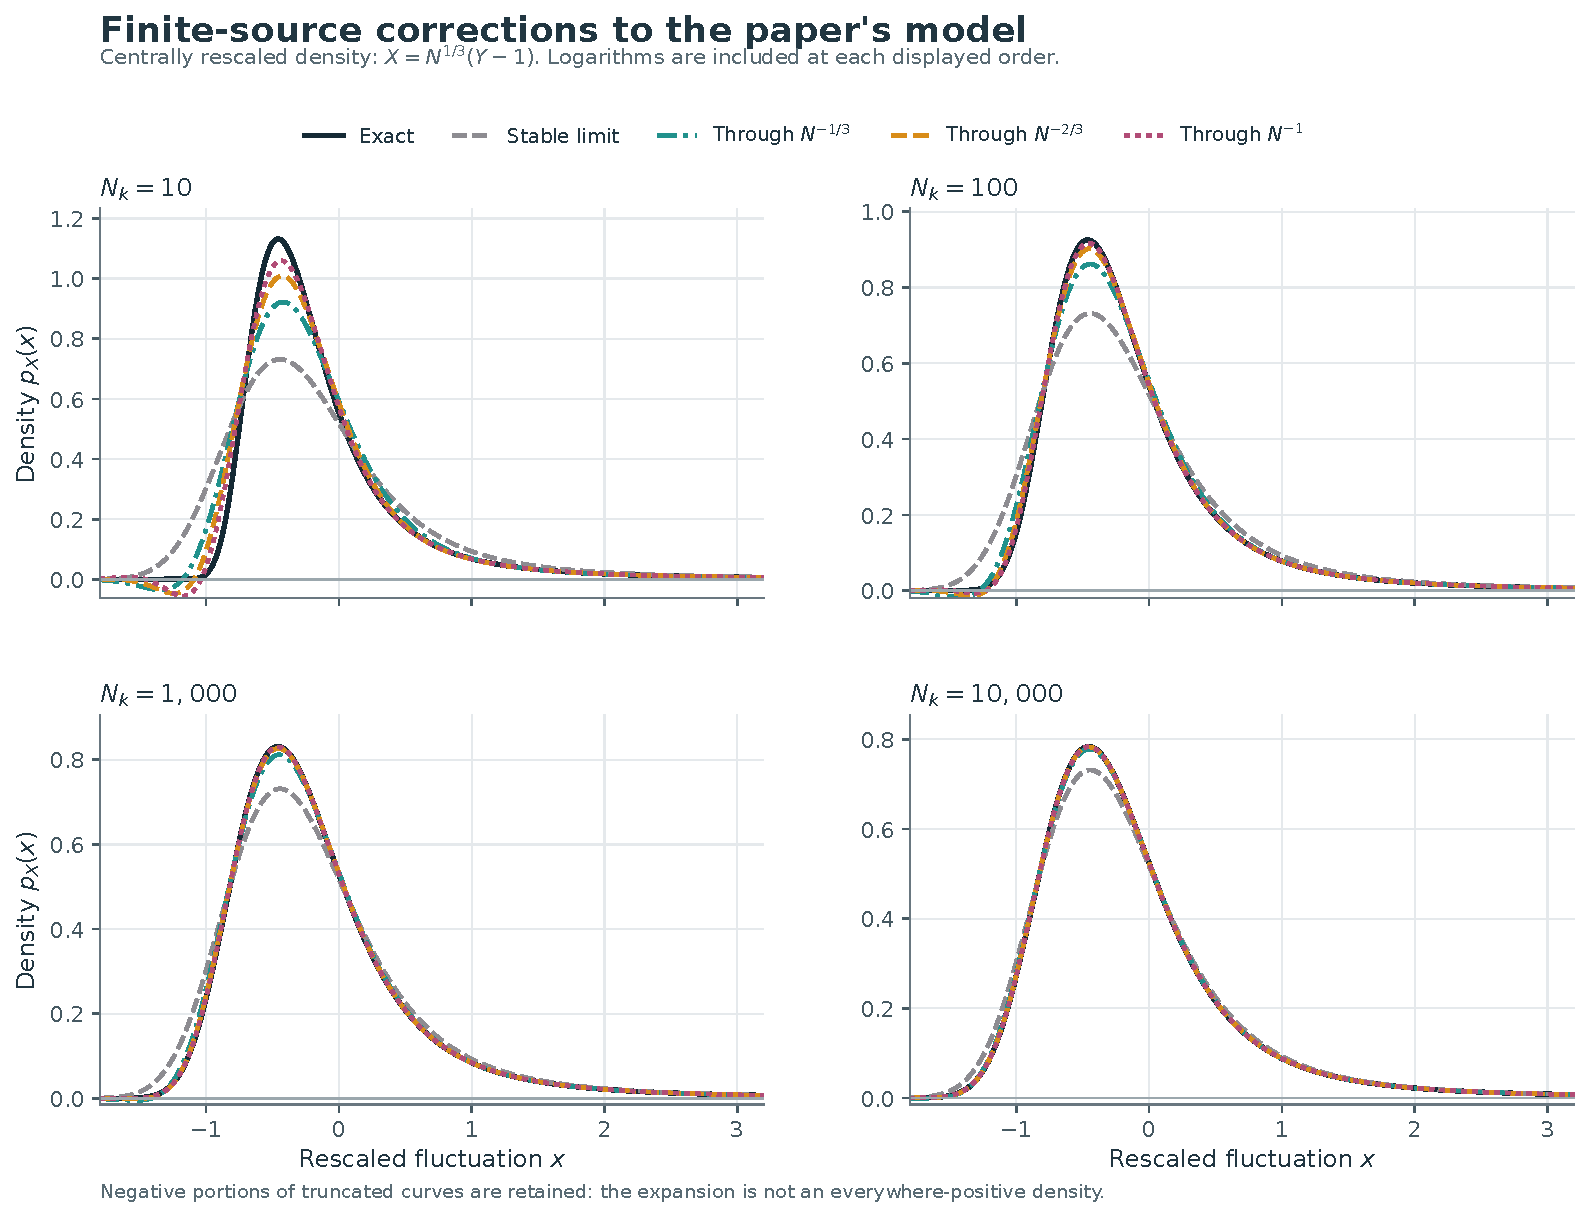
\includegraphics[width=\linewidth]{paper_convergence.pdf}
 \caption{Exact continuous density and successive central expansions for
 the paper's Section V population. The horizontal coordinate is
 $x=N^{1/3}(H/\mu-1)$, so the stable limit is the same curve in every panel.
 Order 3 includes all terms through relative $1/N$, including products of
 lower-order exponent corrections. The left tail is the most demanding
 region, and a finite asymptotic approximation can become negative there.
 Negative values must not be interpreted as probabilities.}
 \label{fig:paperconvergence}
\end{figure}

\section{What additional information is needed for a general population?}
\label{sec:general}

Assume a more general source distribution has
\begin{equation}
 \rho(u)=a u^{-5/2}+b u^{-3}+o(u^{-3}),
 \qquad a=\frac{1}{4\sqrt\pi}.
 \label{eq:generaltail}
\end{equation}
Define the subtracted finite part
\begin{align}
 M_2^{\rm fp}={}&\int_0^1u^2
       [\rho(u)-a u^{-5/2}]\,\dd u\nonumber\\
 &+\int_1^\infty
   \left\{u^2[\rho(u)-a u^{-5/2}]-\frac bu\right\}\,\dd u,
 \label{eq:finitepart}
\end{align}
assuming the subtracted remainder is integrable. Differentiating
Eq.~\eqref{eq:Psi} twice gives
\begin{equation}
 \Psi''(q)=\frac14q^{-1/2}
 +M_2^{\rm fp}-b(\log q+\gE)+o(1).
\end{equation}
Twice integrating with $\Psi(0)=\Psi'(0)=0$ yields
\begin{equation}
 \boxed{\displaystyle
 \Psi(q)=\frac{q^{3/2}}3
 +\frac{q^2}{2}
  \left[M_2^{\rm fp}-b\left(\log q+\gE-\frac32\right)\right]
 +o(q^2).}
 \label{eq:generalcorrection}
\end{equation}
The reference value $u=1$ in the subtraction is a convention: changing it
changes the finite constant and the logarithm together, leaving the exponent
unchanged. For the paper model,
\begin{equation}
 b=-\frac{1}{4\pi},\qquad
 M_2^{\rm fp}=\frac{1-\log(4\pi)}{4\pi},
\end{equation}
which reproduces Eq.~\eqref{eq:paperexpansion}.

If $b=0$ and the ordinary subtracted integral
$M_2^{\rm reg}=\int_0^\infty u^2[\rho(u)-a u^{-5/2}]\,\dd u$ converges,
the first correction simplifies to
\begin{equation}
 p_X(x)=\Pstable(x)
       +\frac{M_2^{\rm reg}}{2N^{1/3}}\Pstable''(x)+\cdots.
 \label{eq:nolog}
\end{equation}
The subtracted coefficient is not a physical variance and may be negative.
The universal mean and leading tail do not determine either $b$ or
$M_2^{\rm fp}$. Higher-order corrections similarly require further tail
coefficients and finite subtracted integrals.

Physically, with inverse-square flux in a locally Euclidean population, a
radial density profile with a linear term at the observer produces an
$S^{-3}$ contribution to the flux distribution and hence a logarithm.
A smooth even radial profile can instead have its first correction at
$S^{-7/2}$. Cosmological evolution and the flux-distance relation also
contribute to subleading tails in a realistic light-cone population.

\section{Four models with the same mean and leading stable law}
\label{sec:models}

We compare four shapes satisfying both Eq.~\eqref{eq:mean} and $F(\infty)=1$.
At a common $N$ they therefore have the same mean $Y=1$, the same leading
bright-source tail, and the same leading density $\Pstable$. Differences in
the exact central densities isolate finite-count model dependence.
The Euclidean examples use identical intrinsic source luminosities; because
$u\propto r^{-2}$, their $F(u)$ is a radial density envelope expressed in
flux coordinates. They are analytic controls rather than observationally
calibrated supermassive-black-hole binary populations.

\subsection{Uniform sphere}
For constant density inside a finite radius, the least luminous observed
source has a minimum flux $u_0$. Mean matching fixes
\begin{equation}
 F_{\rm sphere}(u)=\mathbf1_{u\ge u_0},\qquad u_0=\frac{1}{4\pi}.
\end{equation}
The exact exponent is
\begin{align}
 \Psi_{\rm sphere}(q)={}&q+\frac{q^{3/2}}3\erfc(\sqrt{qu_0})\nonumber\\
 &+\left(\frac{4\pi}{3}-\frac{2q}{3}\right)e^{-qu_0}
 -\frac{4\pi}{3}.
 \label{eq:sphere}
\end{align}
Its small-$q$ expansion is
\begin{equation}
 \Psi_{\rm sphere}(q)=\frac{q^{3/2}}3
 -\frac{q^2}{8\pi}+\frac{q^3}{288\pi^2}+O(q^4).
 \label{eq:sphereexp}
\end{equation}
There is no $q^2\log q$ term, and no $q^{5/2}$ term.

\subsection{Gaussian radial profile}
Take
\begin{equation}
 F_{\rm G}(u)=e^{-c/u},\qquad c=\frac1{16}.
\end{equation}
This represents a Gaussian falloff with distance. More generally,
\begin{equation}
 \Psi_c(q)=\frac{(1+2\sqrt{cq})e^{-2\sqrt{cq}}-1}{8c^{3/2}}
             +\frac{q}{4\sqrt c}.
 \label{eq:gaussiangeneral}
\end{equation}
The mean is $1/(4\sqrt c)$, so $c=1/16$ matches Eq.~\eqref{eq:mean}.
For this value,
\begin{align}
 \Psi_{\rm G}(q)&=8[(1+\sqrt q/2)e^{-\sqrt q/2}-1]+q,
 \label{eq:gaussian}\\
 &=\frac{q^{3/2}}3-\frac{q^2}{16}
   +\frac{q^{5/2}}{120}-\frac{q^3}{1152}+O(q^{7/2}).
 \label{eq:gaussianexp}
\end{align}

\subsection{Two-scale Gaussian mixture}
To vary the distance distribution while retaining analytic control, take
\begin{equation}
 F_{\rm mix}(u)=\frac13e^{-1/(64u)}+\frac23e^{-1/(4u)}.
 \label{eq:mixtureF}
\end{equation}
Both the leading tail and the combined mean remain matched. By linearity of
the Poisson exponent,
\begin{align}
 \Psi_{\rm mix}(q)&=\frac13\Psi_{1/64}(q)
                  +\frac23\Psi_{1/4}(q)\nonumber\\
 &=\frac{q^{3/2}}3-\frac{3q^2}{32}
   +\frac{11q^{5/2}}{480}-\frac{43q^3}{9216}+O(q^{7/2}).
 \label{eq:mixture}
\end{align}

For all three Euclidean controls, use Eq.~\eqref{eq:pdfthird} with
$A=\alpha_2z^2$, $B=\alpha_{5/2}z^{5/2}$, and $C=\alpha_3z^3$.
Their coefficients and literal expected source counts are listed in
Table~\ref{tab:coefficients}. The lack of logarithms does not remove the
fractional ordering of the central expansion.

\begin{table}[tbp]
 \centering
 \caption{Coefficients in
 $\Psi=q^{3/2}/3+\alpha_2q^2+\alpha_{5/2}q^{5/2}+\alpha_3q^3+\cdots$
 for the Euclidean controls. The expected literal count is $\lambda N$.
 The paper model has the logarithmic coefficients in
 Eq.~\eqref{eq:paperexpansion} and an infinite count of arbitrarily faint sources.}
 \label{tab:coefficients}
 \begin{tabular}{lcccc}
 \toprule
 Model & $\alpha_2$ & $\alpha_{5/2}$ & $\alpha_3$ & $\lambda$\\
 \midrule
 Uniform sphere & $-1/(8\pi)$ & $0$ & $1/(288\pi^2)$ & $4\pi/3$\\[0.35em]
 Gaussian & $-1/16$ & $1/120$ & $-1/1152$ & $8$\\[0.35em]
 Two-scale mixture & $-3/32$ & $11/480$ & $-43/9216$ & $22$\\
 \bottomrule
 \end{tabular}
\end{table}

The finite-count models also have an exact atom at zero strain:
$\Pr(H=0)=e^{-\lambda N}$. In the $X$ coordinate this is located at
$x=-N^{1/3}$. The plotted exact curves describe the continuous part.
Even the largest omitted atom, for the sphere at $N=10$, is below
$7\times10^{-19}$, so it is immaterial to these figures. This qualification
matters for extending the calculation to small effective counts.

\begin{figure}[tbp]
 \centering
 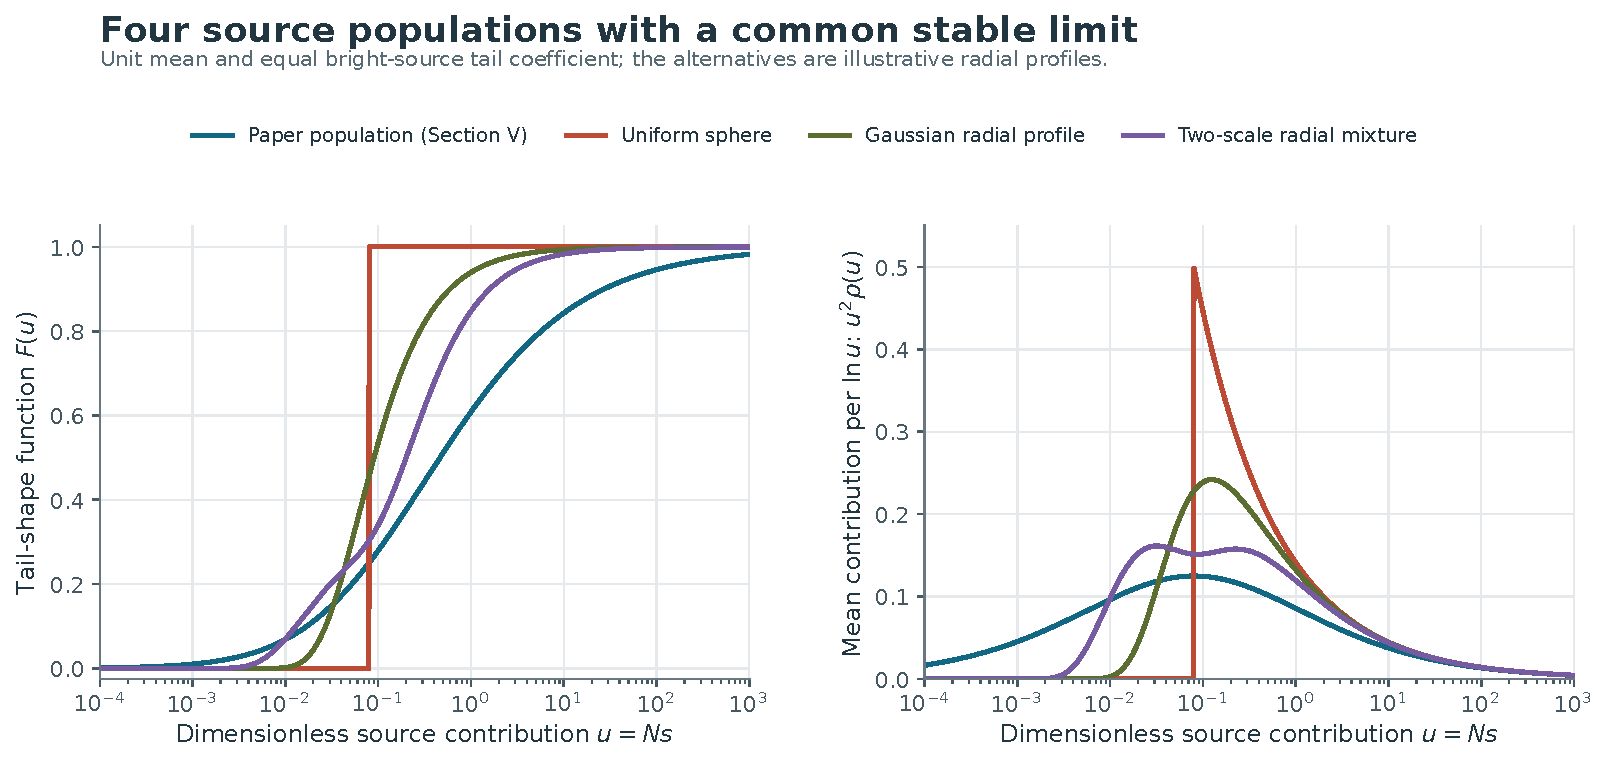
\includegraphics[width=\linewidth]{source_flux_models.pdf}
 \caption{Source-count shapes used in the comparison. The shape factor
 $F(u)$ shows the common large-flux limit and the different faint-source
 populations. The quantity $u^2\rho(u)$ is the mean contribution per
 logarithmic interval in $u$; its integral over $\dd\log u$ is unity for
 every model. The displayed flux range need not contain the entire mean.
 Model differences are therefore compared after matching the full, analytic
 mean and the bright-source coefficient, not by normalizing a plotted window.}
 \label{fig:sourceflux}
\end{figure}

\begin{figure}[tbp]
 \centering
 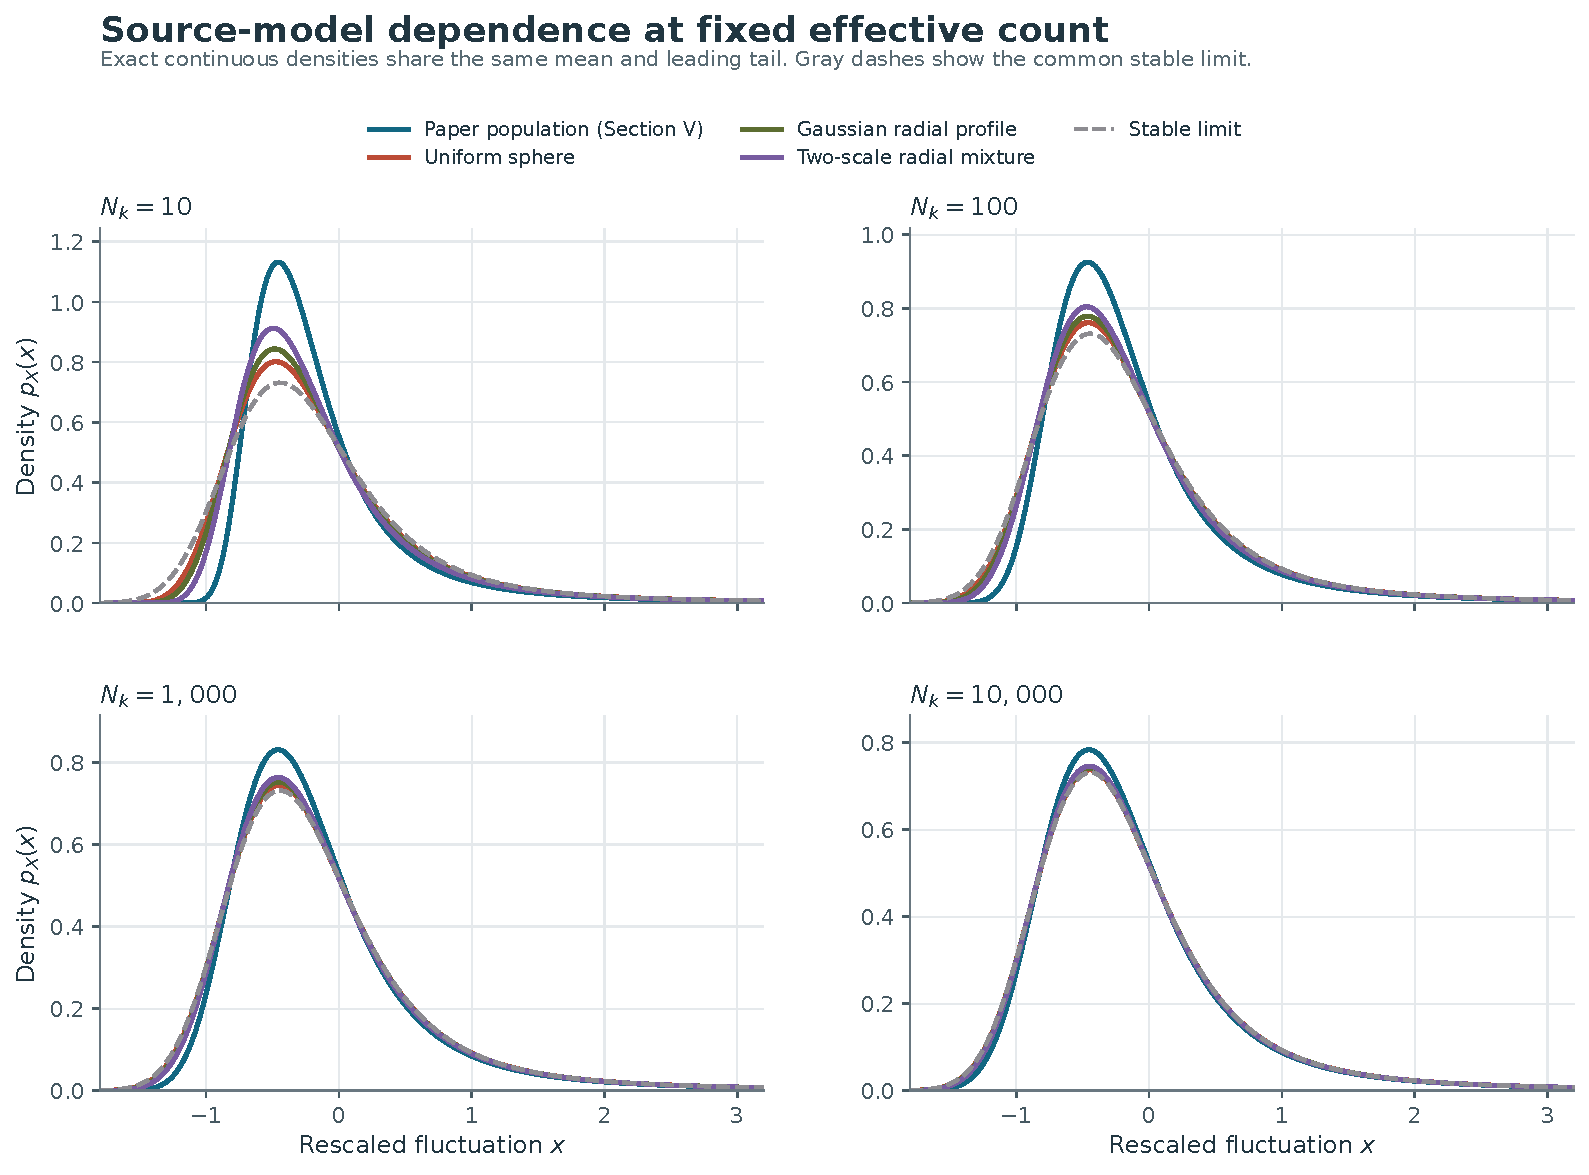
\includegraphics[width=\linewidth]{source_models.pdf}
 \caption{Exact continuous densities for four matched source models at
 different effective counts. Each model has the same $\mu$ and $N$ in a
 panel. All approach the same stable distribution, but their finite-count
 central shapes differ. The paper model has a logarithmic leading correction;
 the three Euclidean controls do not. These models illustrate sensitivity
 to the source distribution and should not be read as alternative fitted
 black-hole population prescriptions.}
 \label{fig:sourcemodels}
\end{figure}

\section{Numerical comparison and interpretation}
\label{sec:numerics}

The numerical procedure evaluates the exact exponent on the imaginary axis
and inverts its characteristic function. Small-argument series avoid the
cancellation in the closed forms, and the stable-weighted integrals in
Eq.~\eqref{eq:pdfthird} give the successive approximations. The numerical
implementation and validation routines accompanying this note specify the
quadrature and sampling choices used for the figures.
The figure defaults use a Fourier grid with spacing $\Delta t=0.02$ and
upper endpoint $t_{\max}=160$. Central error curves use 101 uniformly spaced
points on $-1.5\leq x\leq2$ and 13 logarithmically spaced counts from $10$
through $10^5$. All plotted distributions are deterministic Fourier
inversions; no Monte Carlo sampling enters the calculation.

As a numerical benchmark, Table~\ref{tab:benchmark} compares the paper model
at $N=1000$. The large difference at $x=-1$ illustrates that a moderately
large effective count alone does not guarantee a small relative error on
the low-strain side. The complete expansion through $1/N$ substantially
improves the core.

\begin{table}[tbp]
 \centering
 \caption{Paper model at $N=1000$. Values are densities of $X$, not $Y$ or
 $H$. Order 1 includes the full logarithmic and nonlogarithmic first
 correction; order 3 is Eq.~\eqref{eq:pdfthird}.}
 \label{tab:benchmark}
 \begin{tabular}{rrrrr}
 \toprule
 $x$ & Exact & Stable limit & Order 1 & Order 3\\
 \midrule
 $-1.0$ & 0.23564771 & 0.30234093 & 0.25765642 & 0.23742475\\
 $-0.5$ & 0.82661729 & 0.72618018 & 0.80623748 & 0.82555695\\
 $ 0.0$ & 0.52904555 & 0.51763881 & 0.53355430 & 0.52931352\\
 $ 1.0$ & 0.08413935 & 0.09292649 & 0.08413723 & 0.08413914\\
 \bottomrule
 \end{tabular}
\end{table}

Figure~\ref{fig:errors} uses central absolute density errors so that very
small exact densities do not dominate the diagnostic through division by
near-zero numbers. The error is evaluated on the sampled interval stated
in the figure, and is not a supremum over all possible strains. For the
paper model, the expected leading hierarchy includes
$N^{-1/3}\log N$, $N^{-2/3}\log^2N$, and $N^{-1}\log^3N$, together with
lower logarithmic powers at each order. For the controls, the corresponding
central ordering is in powers of $N^{-1/3}$ without those logarithms.

The rescaled plots deliberately hide the principal change in physical width.
Figure~\ref{fig:physical} restores the variable $Y=H/\mu$ and the density
$p_Y(y)=N^{1/3}p_X[N^{1/3}(y-1)]$. It makes the narrowing with increasing
$N$ visible, while retaining the asymmetric high-strain tail. A logarithmic
ordinate spans the central peaks and the much smaller tail densities; it
does not alter the normalization of the curves.

\begin{figure}[tbp]
 \centering
 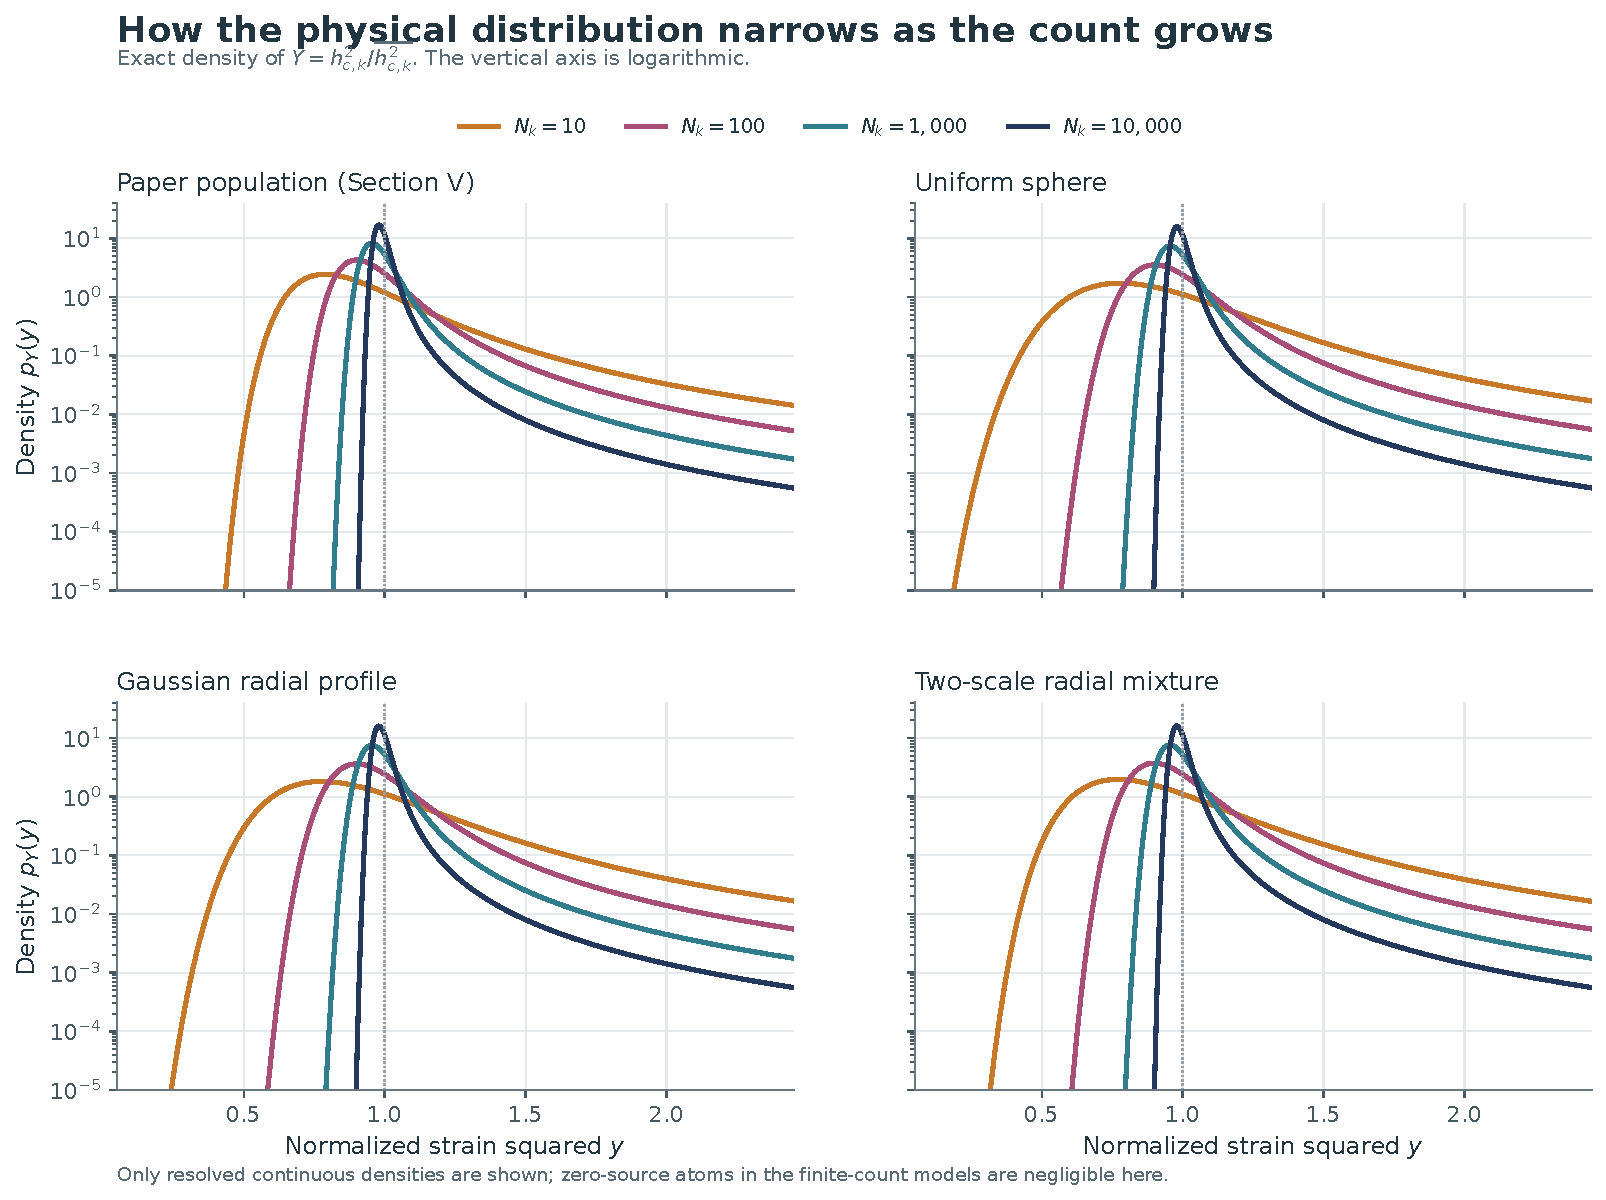
\includegraphics[width=\linewidth]{physical_distributions.pdf}
 \caption{Exact continuous distributions in the physical strain ratio
 $y=h_{c,k}^2/\overline{h_{c,k}^2}$ for $N=10,100,1000,10^4$, shown separately
 for each source model. The ordinate is $p_Y(y)$ on a logarithmic scale.
 Unlike the rescaled $p_X$ curves, these display the decreasing relative
 width and increasing peak height directly. The mean remains $y=1$ for
 every curve, while the mode lies below it.}
 \label{fig:physical}
\end{figure}

\begin{figure}[tbp]
 \centering
 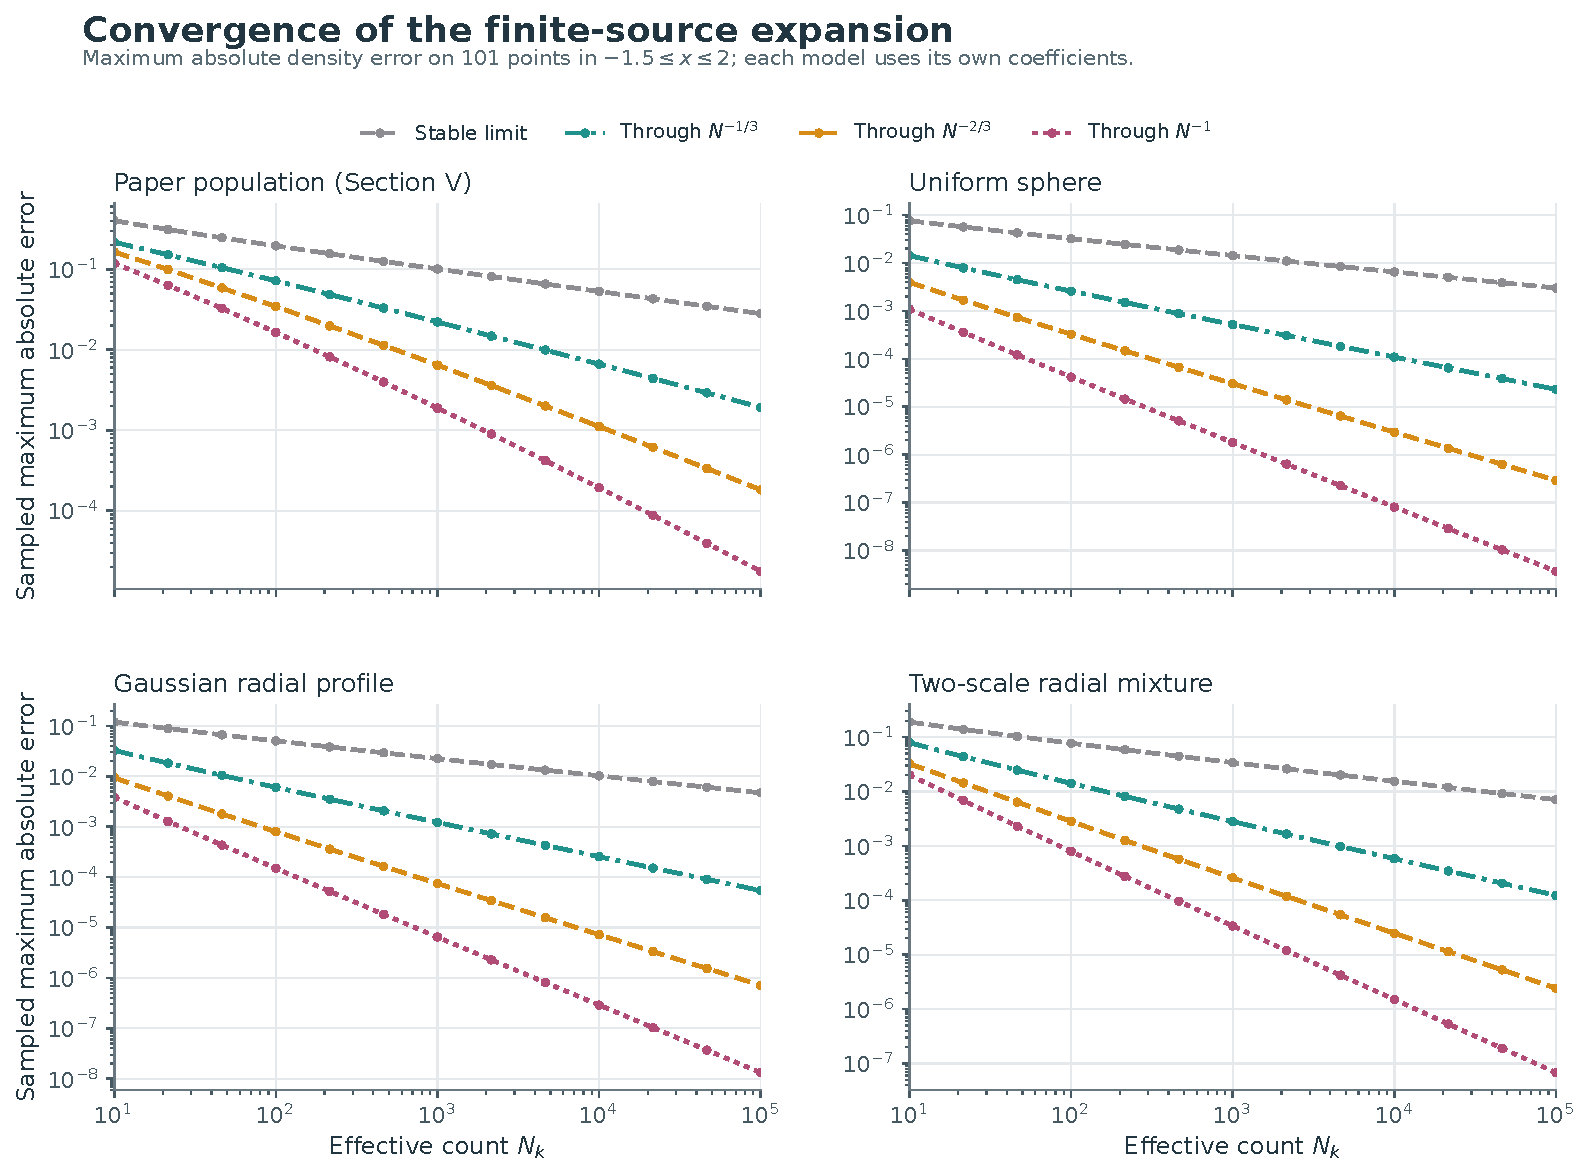
\includegraphics[width=\linewidth]{convergence_errors.pdf}
 \caption{Sampled central absolute errors of successive approximations
 relative to the exact continuous density. The sampling range and numerical
 order convention are specified on the figure. Improved central convergence
 does not establish uniform relative accuracy in the far left tail, nor
 does it guarantee positivity of a finite truncation.}
 \label{fig:errors}
\end{figure}

For practical likelihood use, a negative asymptotic tail should trigger use
of the exact exponent or a separately validated positive approximation.
Clipping the expansion at zero changes its normalization and moments and is
not part of this derivation. Likewise, exponentiating a truncated correction
outside the stable Fourier factor can give an uncontrolled high-frequency
integrand; Eq.~\eqref{eq:pdfthird} expands the characteristic function
consistently before inversion.

\section{Scope and reproducibility}

This calculation concerns the single-band distribution of the latent
squared strain under independent Poisson source counts. It does not derive
the full joint distribution of pulsar timing residuals, inter-band
correlations from eccentric harmonics, or changes induced by a
selection-dependent removal of bright sources. The framework can use a
different source intensity, but the small-$q$ coefficients must then be
rederived.

The repository contains the LaTeX source and bibliography, the numerical
source-model implementation, the figure-generation scripts, generated figure
files, and tabulated numerical results. The repository README gives exact
commands to recreate the plots and compile this note. Figures compare
specified analytic populations without fitting external data. The original
paper supplies the stable limit and its explicit Section~V population; the
finite-count derivations and the matched-model comparisons above are the
extensions developed here.

\bibliographystyle{plainnat}
\bibliography{references}
\end{document}
